\section{Casos de Uso}
A partir de los requerimientos ya definidos, se desarrolla el diagrama de casos de uso, en el que se representan las interacciones entre actores y las partes más importantes del software a desarrollar. Luego, se realizan las especificaciones de los casos de uso definidos en el diagrama.
\subsection{Diagrama de Casos de Uso}
\begin{figure}[H]
	\centering
	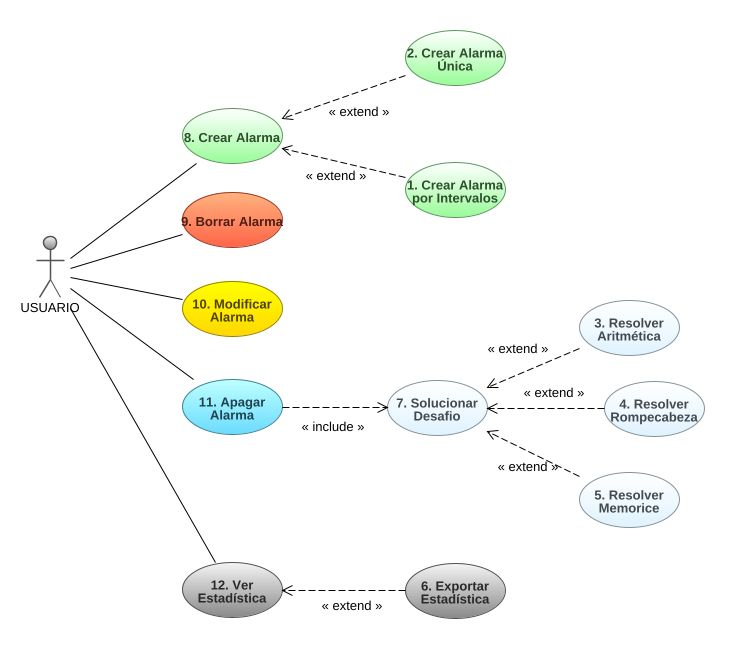
\includegraphics[width=\textwidth]{img/Diagrama Casos de Uso.jpg}
	\caption{Diagrama de Casos de Uso}
	\label{fig:Diagrama de Casos de Uso}
\end{figure}
\newpage

\subsection{Especificación de Casos de Uso}
En esta sección se presenta la especificación de los casos de uso introducidos por el diagrama de casos de uso.

\begin{table}[H]
    \centering
    \caption{Caso de Uso Nº1: }
    \begin{tabular}{| p{0.4\linewidth} | p{0.4\linewidth} |}
        \hline
        \multicolumn{2}{|l|}{\textbf{Caso de Uso Nº1:}  Crear alarma por intervalos} \\
        \hline
        \multicolumn{2}{|l|}{\textbf{Resumen:}  El usuario crea una alarma dentro de un intervalo de tiempo.} \\
        \hline
        \multicolumn{2}{|l|}{\textbf{Frecuencia:}  Ilimitada} \\
        \hline
        \multicolumn{2}{|l|}{\textbf{Actores:}  Usuario} \\
        \hline
        \multicolumn{2}{|l|}{\textbf{Precondiciones:}} \\
        \hline
        \multicolumn{2}{|l|}{\textbf{Descripción del flujo normal (escenario exitoso)} } \\
        \hline
        \textbf{Responsabilidad del actor} & \textbf{Responsabilidad del sistema}\\
         & 1. Habilitar campo “Hora inicio”.\\
         & 2. Habilitar campo “Hora término”. [exc01]\\
         & 3. Habilitar campo “Frecuencia”. \\
         4. Ingresar “Hora inicio”. \\
         5. Ingresar “Hora término”. \\
        6. Ingresar “Frecuencia”. \\ & 7. Habilitar opción “Desafío aritmético”.\\
         & 8. Habilitar opción “Desafío rompecabeza”.\\
         & 9. Habilitar opción “Desafío memoriec”.\\
        10. Seleccionar una de las opciones (“Desafío aritmético”, “Desafío rompecabeza”, “Desafío memoriec”) & \\
         & 11. Habilitar opción “ingresar intervalo”\\
        12. Seleccionar la opción “Ingresar intervalo”.\\
         & 13. Crear alarma por intervalos [exc02]\\
         & 14. Fin del caso de uso \\
        \hline
        \multicolumn{2}{|p{0.8\linewidth}|}{\textbf{[exc01]:} Intervalo incorrecto. Se muestra un mensaje de advertencia “la hora de término tiene que ser mayor a la de inicio”.} \\
        \multicolumn{2}{|p{0.8\linewidth}|}{\textbf{[exc02]:} Alarma ya existente. Se muestra un mensaje de advertencia “La alarma ya existe”.} \\
        \hline
        \multicolumn{2}{|l|}{\textbf{Poscondición:}  Alarma creada por intervalos.} \\
        \hline
    
    \end{tabular}    
    
    \label{table:1}
\end{table}

\begin{table}[H]
    \centering
    \caption{Caso de Uso Nº2: }
    
    \begin{tabular}{| p{0.4\linewidth} | p{0.4\linewidth} |}
        \hline
        \multicolumn{2}{|l|}{\textbf{Caso de Uso Nº2:} Crear alarma única} \\
        \hline
        \multicolumn{2}{|l|}{\textbf{Resumen:} El usuario crea una alarma para una hora exacta.} \\
        \hline
        \multicolumn{2}{|l|}{\textbf{Frecuencia:} Ilimitada} \\
        \hline
        \multicolumn{2}{|l|}{\textbf{Actores:} Usuario} \\
        \hline
        \multicolumn{2}{|l|}{\textbf{Precondiciones:}} \\
        \hline
        \multicolumn{2}{|l|}{\textbf{Descripción del flujo normal (escenario exitoso)} } \\
        \hline
        \textbf{Responsabilidad del actor} & \textbf{Responsabilidad del sistema} \\
        & 1. Habilitar campo “Hora Alarma”. \\
        2. Ingresar “Hora Alarma”. &\\
        & 3. Habilitar opción “Desafío aritmético”. \\
        & 4. Habilitar opción “Desafío rompecabeza”. \\
        & 5. Habilitar opción “Desafío memoriec”. \\
        6. Seleccionar una de las opciones (“Desafío aritmético”, “Desafío rompecabeza”, “Desafío memoriec”) & \\
        & 7. Habilitar opción “Ingresar Alarma”. \\
        8. Seleccionar la opción “Ingresar Alarma”. &\\
        & 9. Crear alarma [exc01]. \\
        & 10. Fin del caso de uso \\
        \hline
        \multicolumn{2}{|p{0.8\linewidth}|}{\textbf{[exc01]:} Alarma ya existente. Se muestra un mensaje de advertencia “La alarma ya existe”.} \\
        \hline
        \multicolumn{2}{|l|}{\textbf{Poscondición:} Alarma creada.} \\
        \hline
    \end{tabular}

    \label{table:2}
\end{table}

\begin{table}[H]
    \centering
    \caption{Caso de Uso Nº3: Resolver Aritmética}
    \begin{tabular}{| p{0.4\linewidth} | p{0.4\linewidth} |}
        \hline
        \multicolumn{2}{|l|}{\textbf{Caso de Uso Nº3:}  Resolver Aritmética} \\
        \hline
        \multicolumn{2}{|l|}{\textbf{Resumen:}  El usuario resuelve un desafío aritmético.} \\
        \hline
        \multicolumn{2}{|l|}{\textbf{Frecuencia:}  Ilimitada} \\
        \hline
        \multicolumn{2}{|l|}{\textbf{Actores:}  Usuario} \\
        \hline
        \multicolumn{2}{|l|}{\textbf{Precondiciones:}} \\
        \hline
        \multicolumn{2}{|l|}{\textbf{Descripción del flujo normal (escenario exitoso)} } \\
        \hline
        \textbf{Responsabilidad del actor} & \textbf{Responsabilidad del sistema}\\
            & 1. Mostrar operación aritmética a resolver.\\
            & 2. Habilitar el campo ``solución".\\
        3. Ingresar solución. &\\
            & 4. Habilitar la opción ``ingresar".\\
        5. Aceptar la opción ``Ingresar". &\\
        6. Verificar la solución.[exc01]&\\
        \hline
        \multicolumn{2}{|p{0.8\linewidth}|}{\textbf{[exc01]:} El usuario ingresa una solución incorrecta. El sistema muestra un mensaje de advertencia "solución incorrecta".} \\
        \hline
        \multicolumn{2}{|l|}{\textbf{Poscondición:}  Aritmética resuelta.} \\
        \hline
    \end{tabular}
    \label{table:3}
\end{table}

\begin{table}[H]
    \centering
    \caption{Caso de Uso Nº4: }
    
    \begin{tabular}{| p{0.4\linewidth} | p{0.4\linewidth} |}
        \hline
        \multicolumn{2}{|l|}{\textbf{Caso de Uso Nº4:} Resolver Rompecabezas} \\
        \hline
        \multicolumn{2}{|l|}{\textbf{Resumen:} El usuario resuelve un desafío de rompecabeza.} \\
        \hline
        \multicolumn{2}{|l|}{\textbf{Frecuencia:} Ilimitada} \\
        \hline
        \multicolumn{2}{|l|}{\textbf{Actores:} Usuario} \\
        \hline
        \multicolumn{2}{|l|}{\textbf{Precondiciones:}} \\
        \hline
        \multicolumn{2}{|l|}{\textbf{Descripción del flujo normal (escenario exitoso)} } \\
        \hline
        \textbf{Responsabilidad del actor} & \textbf{Responsabilidad del sistema} \\
        & 1. Mostrar rompecabezas a resolver. \\
        2. Mover piezas del rompecabezas. \\
        & 3. Habilitar la opción “Listo” \\
        4. Seleccionar la opción “Listo”. \\
        & 5. Verificar la solución. [exc01] \\
        & 6. Fin del caso de uso \\
        \hline
        \multicolumn{2}{|p{0.8\linewidth}|}{\textbf{[exc01]:} El usuario ingresa la solución incorrecta. El sistema muestra un mensaje de advertencia “solución incorrecta”.} \\
        \hline
        \multicolumn{2}{|l|}{\textbf{Poscondición:} Rompecabezas resuelto.} \\
        \hline
    \end{tabular}

    \label{table:4}
\end{table}

\begin{table}[H]
    \centering
    \caption{Caso de Uso Nº5: }
    
    \begin{tabular}{| p{0.4\linewidth} | p{0.4\linewidth} |}
        \hline
        \multicolumn{2}{|l|}{\textbf{Caso de Uso Nº5:}  Resolver Memorice} \\
        \hline
        \multicolumn{2}{|l|}{\textbf{Resumen:}El usuario resuelve un desafío de memorice.} \\
        \hline
        \multicolumn{2}{|l|}{\textbf{Frecuencia:}  Ilimitada} \\
        \hline
        \multicolumn{2}{|l|}{\textbf{Actores:}  Usuario} \\
        \hline
        \multicolumn{2}{|l|}{\textbf{Precondiciones:}} \\
        \hline
        \multicolumn{2}{|l|}{\textbf{Descripción del flujo normal (escenario exitoso)} } \\
        \hline
        \textbf{Responsabilidad del actor} & \textbf{Responsabilidad del sistema}\\
            & 1. Mostrar Memorice a resolver.\\
            & 2. Habilitar cartas. \\
            & 4. Verificar solución \\
            & 6. Fin caso de uso. \\
        3. Seleccionar cartas.[exc01] &\\
        5. Volver al paso 3 hasta que esten todas las cartas volteadas &\\
        \hline
        \multicolumn{2}{|p{0.8\linewidth}|}{\textbf{[exc01]:} El usuario voltea cartas distintas. El sistema voltea las cartas boca abajo.} \\
        \hline
        \multicolumn{2}{|l|}{\textbf{Poscondición:}  Memorice resuelto.} \\
        \hline
    \end{tabular}

    \label{table:5}
\end{table}

\begin{table}[H]
    \centering
    \caption{Caso de Uso Nº6: }
    


    \label{table:6}
\end{table}

\begin{table}[H]
    \centering
    \caption{Caso de Uso Nº7: }
    


    \label{table:7}
\end{table}

\begin{table}[H]
    \centering
    \caption{Caso de Uso Nº8: }
    


    \label{table:8}
\end{table}

\begin{table}[H]
    \centering
    \caption{Caso de Uso Nº9: }
    


    \label{table:9}
\end{table}

\begin{table}[H]
    \centering
    \caption{Caso de Uso Nº10: }
    


    \label{table:10}
\end{table}

\begin{table}[H]
    \centering
    \caption{Caso de Uso Nº11: }
    


    \label{table:11}
\end{table}

\begin{table}[H]
    \centering
    \caption{Caso de Uso Nº12: }
    

    
    \label{table:12}
\end{table}